\section{Evaluation}
\label{sec:evaluation}
We evaluate our split and merge error detection and correction recommendation in the context of interactive proofreading tools: to direct users to regions with a high probability of error and to suggest corrections (Fig.~\ref{fig:results}). For comparison, we take publicly available mouse cortex data of the same kind as our training data. This data is part of the ISBI 2013 challenge training dataset ($1024\times1024\times100$ voxels) which was acquired using a serial section scanning electron microscope (ssSEM) with a resolution of $6\times6\times30\, nm$ per voxel. We use the available manually-labeled ground truth to score our approach using the variation of information (VI) metric, which is closely related to mutual information. VI is a measure of the distance between two clusterings, where lower VI numbers are better. Since our classifiers are trained on 2D image slices, we perform all evaluations on slices rather than 3D volumes.

\paragraph{Interactive proofreading.}
Recently, Haehn et al.~discussed requirements for interactive proofreading and evaluated three different tools on connectomics data in a study with naive users~\cite{haehn_dojo_2014}. This study asked users to spend 30 minutes proofreading with the different tools, to correct split and merge errors to improve the automatic segmentation. The best performing tool in their evaluation was Dojo. We use their findings and their user-generated proofreading result data, which they kindly provided, as a baseline for the evaluation of our method.
%The authors performed a non-expert user study and stated that their software Dojo provides better results than other tools due to a minimalistic user interface and sophisticated 3D volume rendering.
%Haehn et al. perform their user study on the most representative sub-volume ($400\times400\times10$ voxels) in terms of distribution of object size. For optimal comparison, we use exactly the same data.

To compare against Dojo, we simulate a user for proofreading correction. We assume that all classification has been computed ahead of time, and that the user is presented with a stream of error corrections to assess. The assessment is simulated by comparing the VI before and after each performed correction. Corrections are accepted only when VI reduces, and we test this across different user error rates (Fig.~\ref{fig:results}). In Haehn et al., the proofreading time was limited to 30 minutes, and human participants performed 59 corrections on average ($\approx30$ seconds per correction). In our scenario, users do not need to visually find errors and manually correct them, and so instead we assume each correction assessment takes 15 seconds (120 assessments in 30 minutes). Split errors are likely to take less time than this; however, merge errors are harder to assess, as the user must select between the top 5 candidate boundaries. Since the performance between human participants of Haehn et al.'s user study shows large variation, we present both the best performing user (VI improvement $.0598$) and the average performance among all users (VI improvement $-0.012$) as our baseline. In the simulated case, the VI improvement in comparison to the ground truth is \VKF{update $0.11$} (Fig.~\ref{fig:results}).

\paragraph{Automatic correction.} As a comparison, we also perform automatic correction. During training, we define a probability threshold $p_t=.95$ \VKF{This is actually different than the 0.7 claimed before} for automatic split correction based on CNN probability from the test set. Then, for automatic correction, we apply both classifiers to produce lists of split and merge errors sorted by confidence. First, we correct merge errors with $\max(1-p)$, followed by split error correction using $p_t$. The total time for the correcting all \JT{\#} errors was 17 minutes (\JT{\#} merge error correction 15min, \JT{\#} split error correction 2min). The average VI improvement in comparison to the ground truth was negative\VKF{update} (Fig.~\ref{fig:results}). This is not surprising, as the problem is very challenging, and this motivates the need for human-in-the-loop proofreading tools.

%\paragraph{Random proofreading.} Given the automatic result, we decided to test a classifier with random performance in comparison to our learned CNN. For split errors, the simulated user is presented with randomly picked boundaries, which they can accept or reject. For merge errors, the simulated user is presented with 5 randomly selected boundaries from the interior of the segmented region. The significantly worse performance of this approach demonstrates that our network is informative to the user.

\begin{figure}[t]
\centering
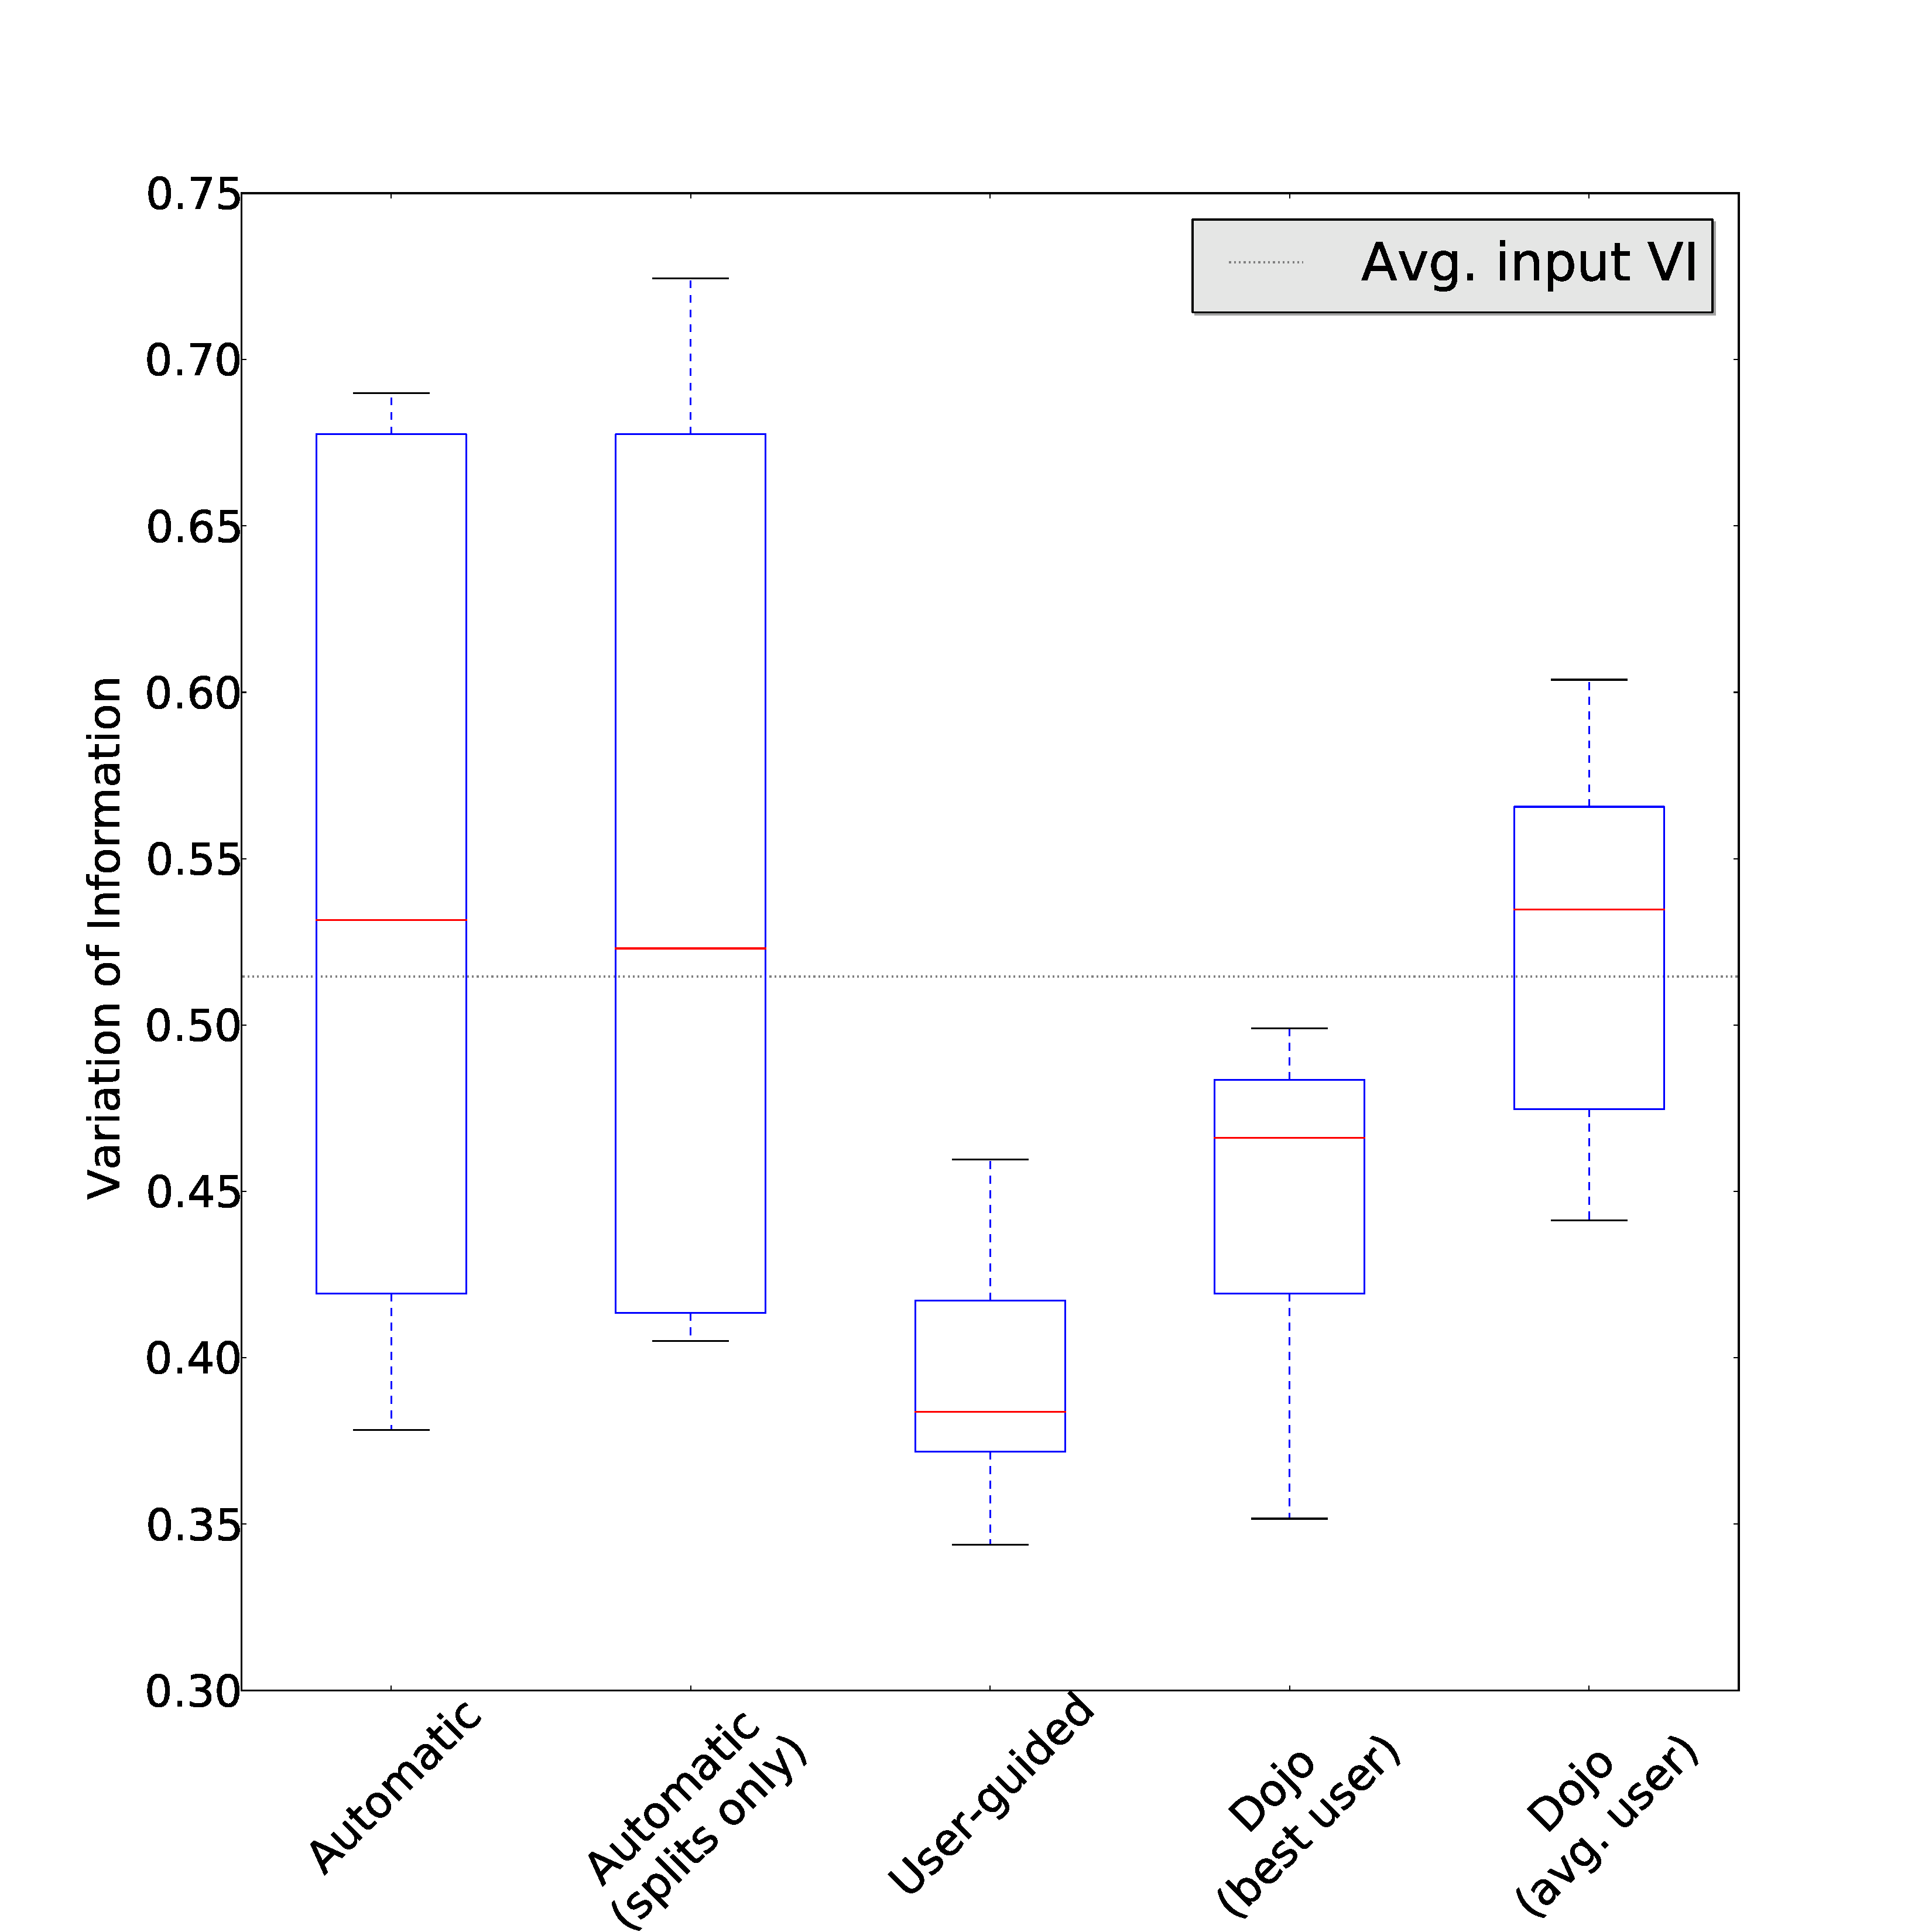
\includegraphics[scale=.1]{gfx/results_new.pdf}
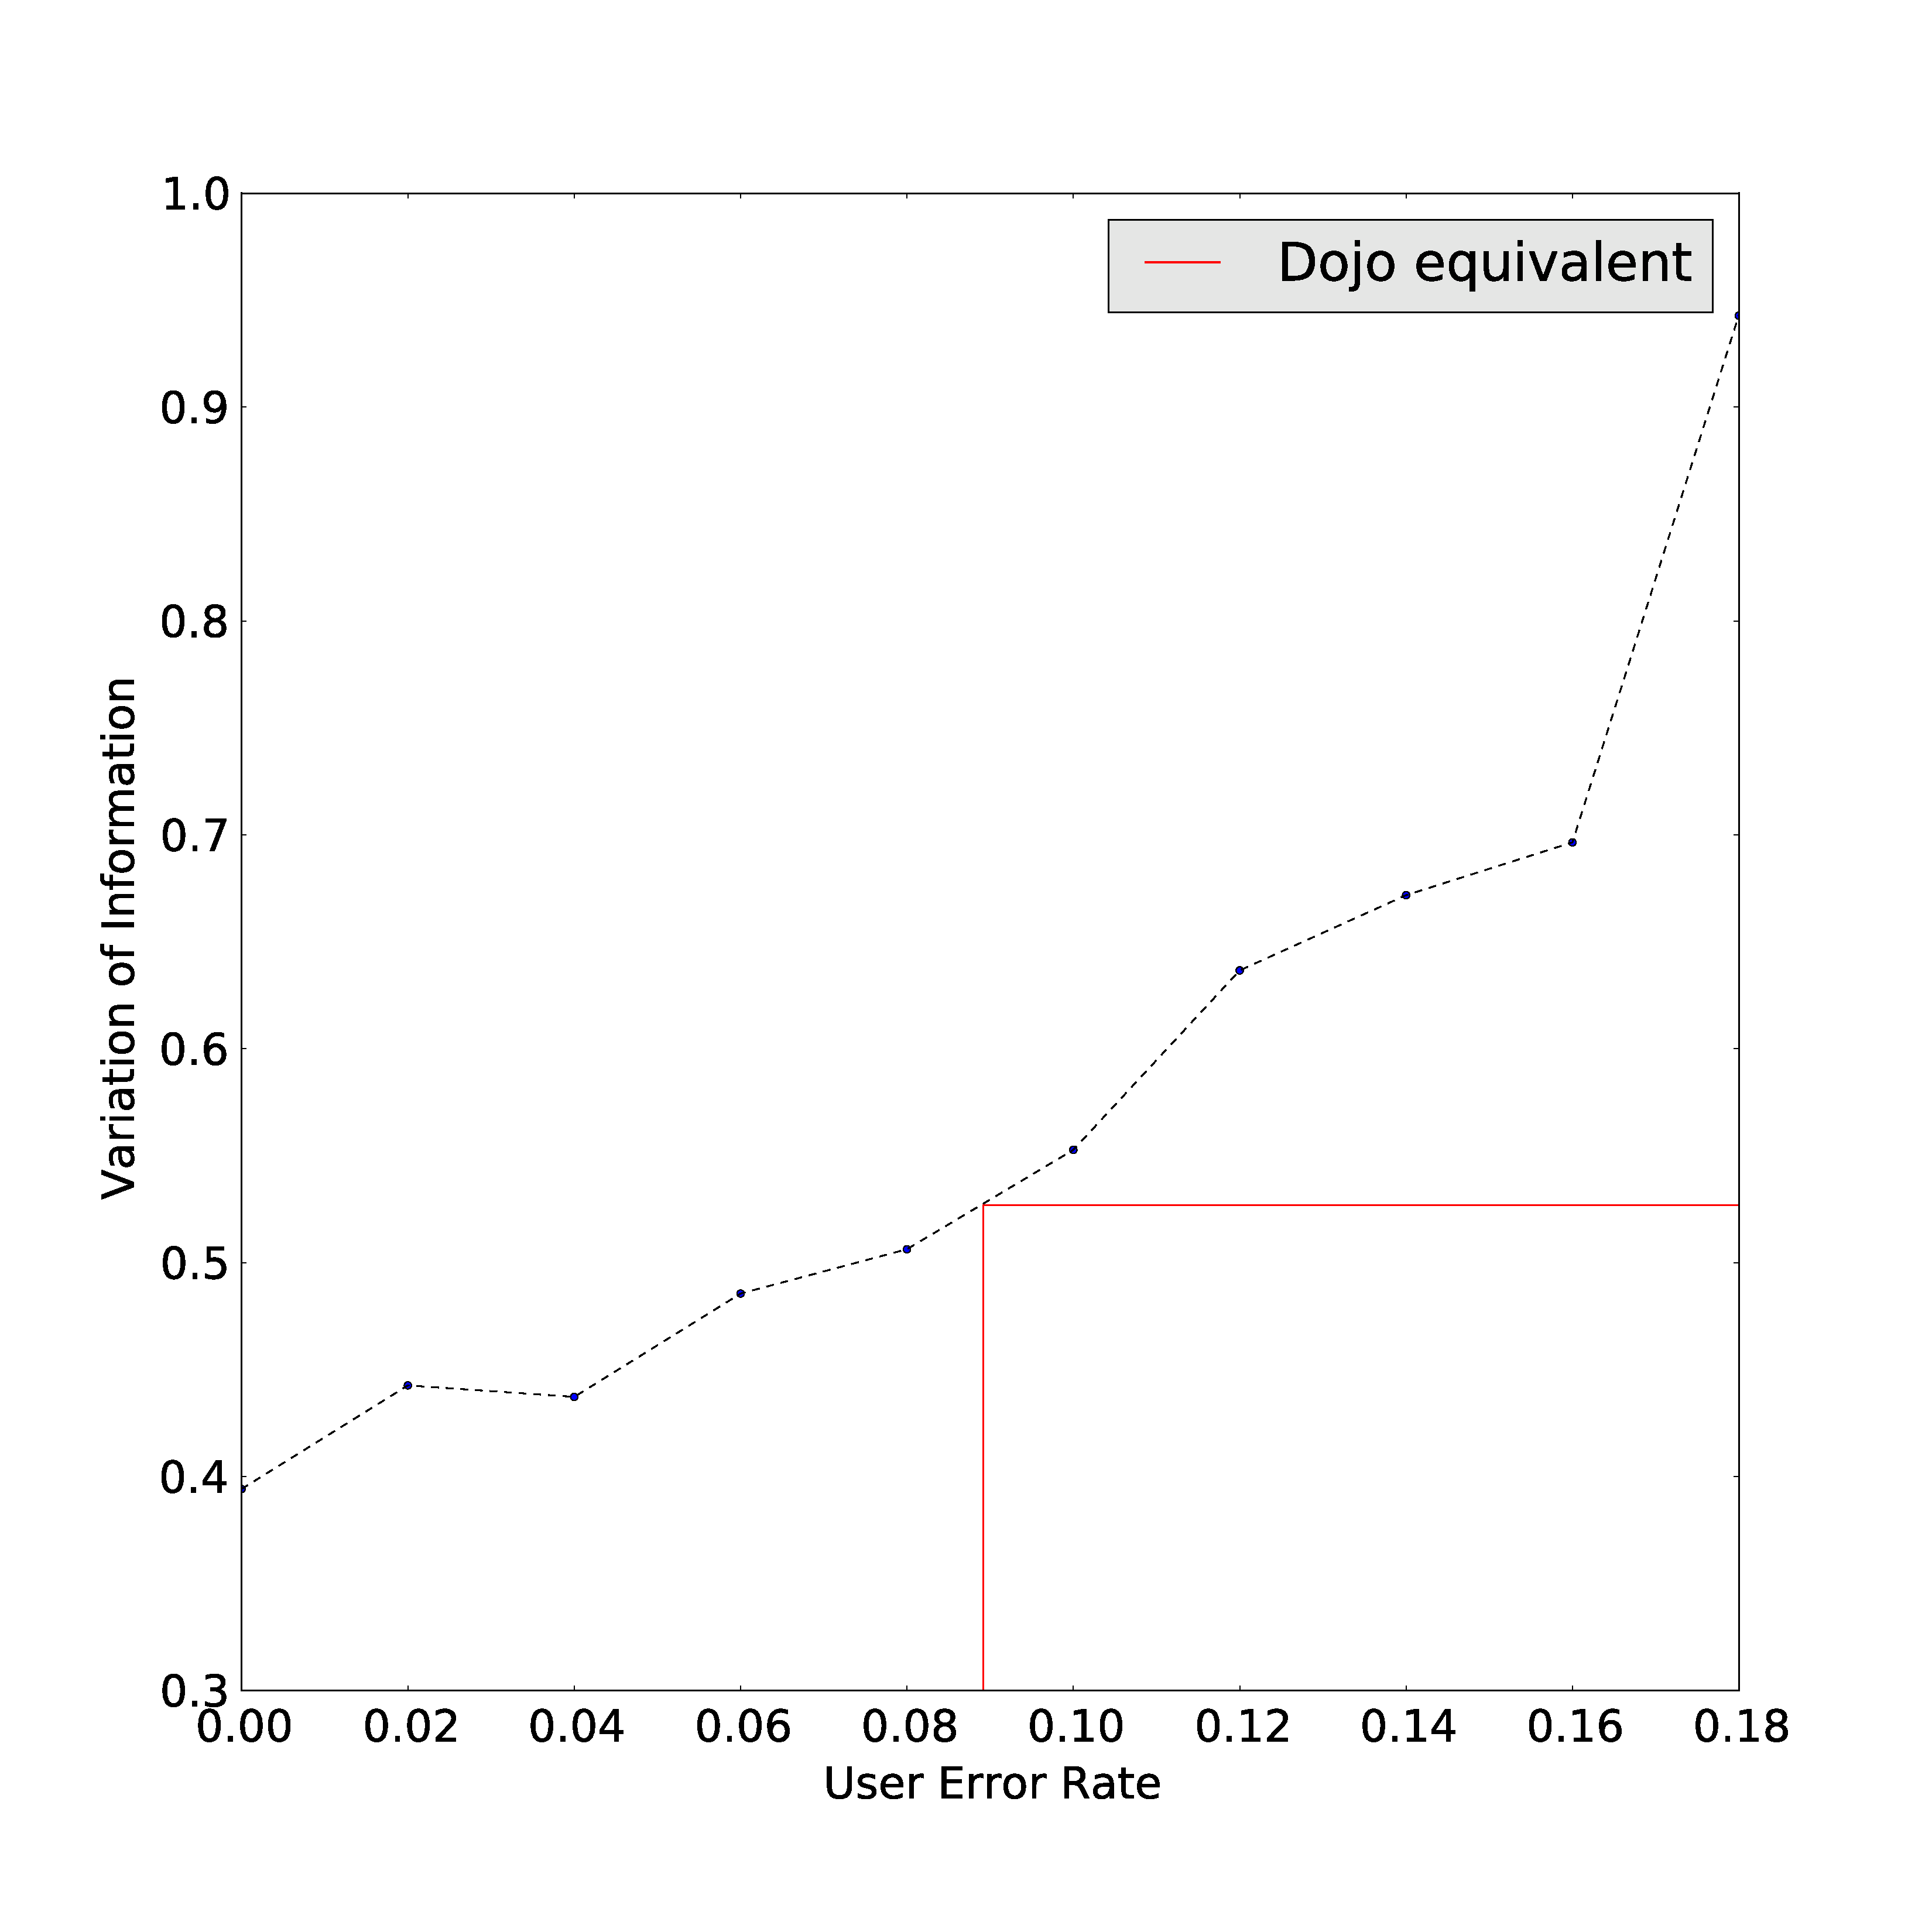
\includegraphics[scale=.1]{gfx/user_error_rate.pdf}
\caption{We compare user-guided (error rate 0.0) and automatic (full+just splits) proofreading results using our trained network,  as well as results from Haehn et al.'s comparison study \cite{haehn_dojo_2014} across 2D slices of connectomics data. The score is measured in variation of information (VI) between an input and the corresponding performance. Lower scores are better.}
\label{fig:results}
\end{figure}
%
%
%\subsection{Split error evaluation}
%
%Paragraph: What is the process of evaluating split errors?
%
%Paragraph: What do we compare against? What is the result? Why is the performance better?
%
%\begin{table}[t]
%\begin{tabular}{ll}
%\toprule
%Method & VI improvement after fixing split errors \\
%\midrule
%Jain design & \\
%Jain design variation & \\
%Our design &  \\
%Our design variation & \\
%\bottomrule
%\end{tabular}
%\caption{This is a table of results. It shows the comparison to Jain et al., and the comparison to different variations of these algorithms with the varying overlap regions.}
%\label{tab:spliterrorcorrectionperformance}
%\end{table}
%
%\subsubsection{Analysis}
%
%Paragraph: Demonstration of ROC curves for VI performance in split error adjustment as the threshold varies.
%
%\begin{figure}[t]
%\missingfigure{}
%\caption{What does the performance of split error correction look like (ROC curve) as the threshold on edge probability changes?}
%\end{figure}
%
%\subsection{Merge error evaluation}
%
%Merge errors are not that common. False positive rate is very important. Choosing threshold is important.
%
%Paragraph: What is the process of evaluating merge errors?
%
%Paragraph: What do we compare against? What is the result? Why is the performance better?
%
%\begin{table}[t]
%\begin{tabular}{ll}
%\toprule
%Method & VI improvement after fixing merge errors \\
%\midrule
%Our design &  \\
%Our design variation & \\
%\bottomrule
%\end{tabular}
%\caption{This is a table of results. It shows our ability to improve VI.}
%\end{table}
%
%
%
%Philosophical point of trading split errors for merge errors...
%
%
%Speed of classification